\newpage \ \thispagestyle{empty} \newpage

\chapter{Motivazioni alla base del tirocinio}
\label{cap:motivazioni-tirocinio}
Questo capitolo si occupa di definire le motivazioni che hanno portato al compimento del percorso di tirocinio curricolare, dal punto di vista aziendale (si propone quella che, a mio parere, è la visione di \textit{\textbf{Trizeta}}) e dal mio punto di vista,
descrivendo i vincoli, gli obiettivi e le esigenze che il progetto proposto punta a soddisfare.

\section{Strategia aziendale}

% In questa sezione descriverò il rapporto che l'azienda ha nei confronti dei tirocini (universitari e non) dal punto di vista delle tecnologie, dei prodotti, del mercato e dal punto di vista di investimento sulle risorse umane.
In base a quanto ho potuto osservare e capire durante il periodo di \textit{stage}, la strategia di gestione dei tirocini curricolari dell'azienda ospitante persegue i seguenti obiettivi:
\begin{itemize}
    \item \glslink{innovazione}{Innovazione}: come riportato al termine della sezione \hyperref[sec:innovazione]{1.4}, l'introduzione di miglioramenti e novità negli strumenti e nelle tecnologie utilizzate (motivata da esigenze produttive o di mercato)
    può avvalersi (come nel mio caso) del parere motivato del tirocinante, tenendo conto del grado di maturità e delle caratteristiche del lavoro svolto per \textit{testare} le novità da introdurre;
    \item \textbf{Integrazione di prodotti esistenti}: il parco \textit{software \textbf{Trizeta}} è vasto ed eterogeneo e la clientela richiede spesso l'implementazione di nuove funzionalità per rispondere a nuove esigenze; un modo per eseguire
        una prima integrazione di tali funzionalità (in versione beta o di \textit{proof of concept}) si basa sul lavoro di uno o più tirocinanti;
        \vspace{-20mm}
        \begin{figure}[H]
            \centering
            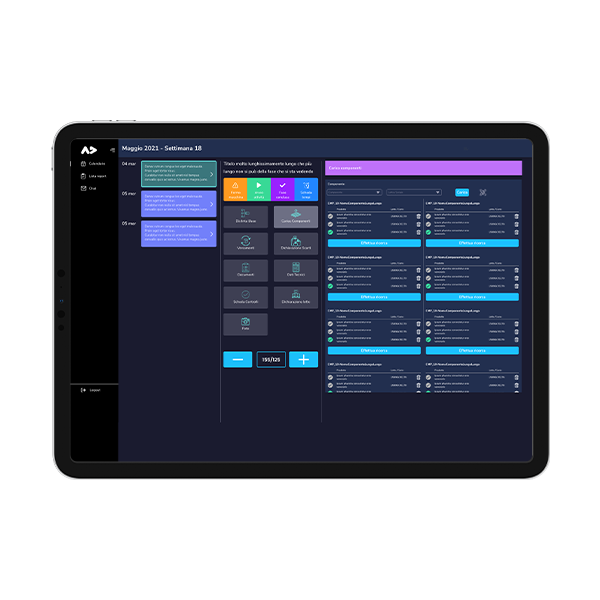
\includegraphics[width=0.8\textwidth]{images/ademes.png}
            \vspace{-20mm}
            \caption[Interfaccia del \textit{software ADeMES}]{Interfaccia del \textit{software ADeMES} \textit{\textbf{Trizeta}}\footnotemark}
        \end{figure}
        \footnotetext{Fonte: \href{https://trizeta.com/ade-mes/}{https://trizeta.com}}
    \item \textbf{Creazione di nuovi prodotti}: in base alle stesse motivazioni espresse al punto precedente, è possibile che la risposta alle nuove esigenze della clientela non sia possibile direttamente all'interno dei prodotti già esistenti (per separazione di ambito o
        per non compromettere la mantenibilità dei prodotti esistenti): in questo caso, concordando lo \glslink{tech-stack}{\textit{stack} tecnologico} da usare, lo \textit{stagista} può implementare un prodotto prototipale \textit{ex-novo} in base alle indicazioni ricevute;
    \item \textbf{Valutazione delle competenze} del tirocinante: il periodo di tirocinio è occasione di introduzione del tirocinante nel contesto aziendale e, per quanto riguarda la mia esperienza, formazione sulla visione aziendale, sui processi in atto, sulle tecnologie utilizzate
        e sulle abilità richieste per l'esecuzione delle attività lavorative; l'azienda ospitante fornisce quindi una formazione di base e valuta quali sono le reazioni agli stimoli (lavorativi e non) in funzione dell'inserimento del tirocinante nel \textit{team} aziendale, data la formazione ricevuta.
        \begin{figure}[H]
            \centering
            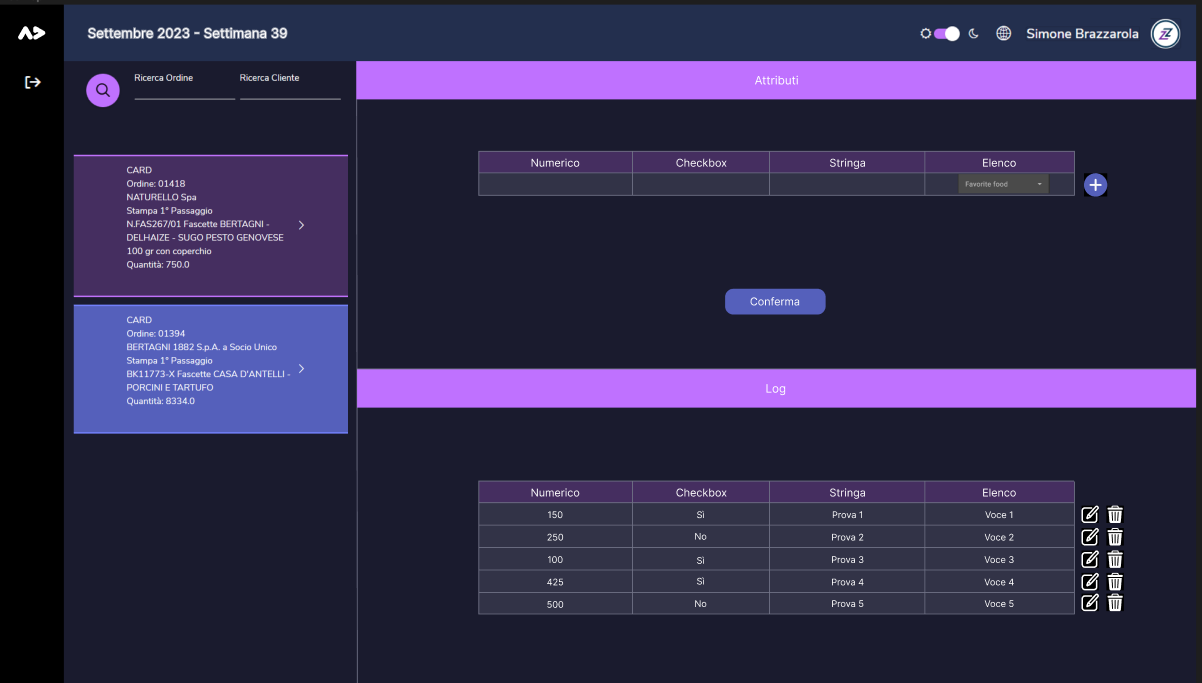
\includegraphics[width=0.8\textwidth]{images/dashboard.png}
            \caption[Interfaccia del prodotto \textit{ADeQA}]{Interfaccia del prodotto \textit{ADeQA}, oggetto del tirocinio}
        \end{figure}
\end{itemize}
\section{Problematiche poste in essere}

% In questa sezione descriverò quali problemi, a livello macroscopico, il prodotto software da me sviluppato ha consentito di superare.
Scopo delle attività di \textit{stage} è la creazione di una \glslink*{pwag}{\textit{progressive web app}} per la raccolta di dati relativi al controllo della qualità delle linee produttive di aziende manifatturiere.
Ogni linea produttiva è costituita da un insieme di "fasi" di lavorazione: ogni fase di lavorazione è considerabile come una \textit{black-box}\footnote{\gls{black-box}} di cui si conoscono gli \textit{input} (materia prima o semilavorati in ingresso)
e gli \textit{output} (semilavorati o prodotti finiti).
\begin{figure}[H]
    \centering
    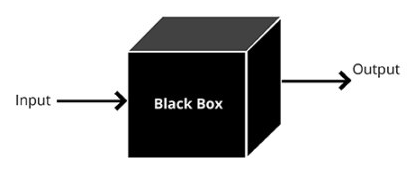
\includegraphics[width=0.6\textwidth]{images/black-box.png}
    \caption[Schema sintesi del concetto di \textit{black-box}]{Schema sintesi del concetto di \textit{black-box}\footnotemark}
\end{figure}
\footnotetext{Fonte: \href{https://www.quora.com/Machine-learning-classifier-is-a-black-box-Why-does-everyone-still-use-it-1}{https://www.quora.com}}
Ogni fase è associata a un insieme di caratteristiche (dette "attributi") relative ai prodotti in uscita dalla stessa: esse sono di interesse per comprendere se la lavorazione ha prodotto articoli utilizzabili nelle fasi successive / nello stoccaggio degli stessi o meno.
Non è noto a priori il numero nè il tipo di attributi associati a una determinata fase di lavorazione: sono tutte informazioni ottenibili tramite l'utilizzo di servizi \textit{backend}\footnote{\gls{backend}} (relativi alla struttura ed alla logica di persistenza) esposti dal tutor aziendale con una
serie di \textit{API\footnote{\gls{apig}} REST\footnote{\gls{restg}}} (astrazioni che consentono di eseguire operazioni sui dati di dominio in una architettura \textit{client - server}).

\section{Obiettivi}

\section{Vincoli}

% In questa sezione descriverò (entrando nei particolari, rispetto alla sezione precedente) le condizioni imposte ed i risultati prefissati.
Il progetto si focalizza quindi sullo sviluppo di codice prettamente \textit{front-end}\footnote{\gls{frontend}}

\section{Scelta del tirocinio}

In questa sezione descriverò le motivazioni che mi hanno portato a scegliere il progetto di tirocinio curricolare, indicando punti a favore e punti a sfavore a monte della scelta.